\section{Auffinden potentieller Barcodes}
\writtenby{\dcauthornameewie}%
Um maschinell lesbar zu sein, zeichnen sich Barcodes durch einen, im Vergleich zur ihrer Umgebung, hohen Helligkeitskontrast aus.
Das im Folgenden beschriebene Verfahren macht sich diesen Umstand zu nutze um Bildregionen zu identifizieren, die mit höherer Wahrscheinlichkeit Barcodes enthalten.
Das Verfahren arbeitet mit einem Graustufenbild \autoref{sec:grayscaling}, das die Helligkeit der Pixel kodiert.

\begin{enumerate}[(1)]
\item \textbf{Kantenbild bestimmen}
Das Kantenbild wird gemäß \autoref{sec:edge-detection} ermittelt.
Der \textsc{Roberts}-Operator erweist sich am geeignetsten da er Bildrauschen weniger stark erfasst als z.B. der \textsc{Sobel}-Operator.

\item \textbf{Kanten verstärken}
Die Kanten werden mit einem $5\times5$ Strukturelement mittels Dilation verstärkt.
Dadurch wird erreicht, dass nah beieinander liegende Kanten (wie es bei Strichcodes der Fall ist) eine möglichst geschloßene Fläche bilden.
Hierbei ist die Wahl der Größe des Strukturelements entscheidend.
Ist es zu klein, bleiben zu große Löcher übrig.
Ist es zu groß kann es vorkommen, dass Barcodes mit geringem Abstand zueinander zu einer Fläsche verschmelzen (trotz vorhandener Ruhezone).

\item \textbf{Segmentierung}
Die Segmentierung erfolgt mittels Thresholding.
Als Schwellwert dient der Mittelwert der Helligkeit aller Bildpunkte.
Die Verwendung des Mittelwertes ist ideal, da sich Kantenpixel durch ihren Gradienten bereits deutlich vom Hintergrund abzeichnen.
Das Resultat ist ein Binärbild mit Hintergrund in schwarz (0\%) und Bildelementen in weiß (100\%).

\item \textbf{Komponenten extrahieren}
Wie in \autoref{sec:connected-components} beschrieben, werden die zusammenhängenden Komponenten der Bildelemente extrahiert.
Punktmengen stellen die resultierenden Komponenten dar.

\item \textbf{Regionen klassifizieren}
Die extrahierten Komponenten beschreiben bisher nur Bildelemente mit erhöhtem Kontrast.
Darunter fallen, neben den erwünschten Barcodes, auch Elemente wie z.B. Schrift und Symbole.
Um alle potentiellen Barcodes auszuwählen sind alle Komponente, die nicht als Barcode in Frage kommen, herauszufiltern.

Es hat sich gezeigt, dass Regionen, denen Barcodes entsprechen, sich dadurch auszeichnen, dass deren Komponenten deutlich geschloßener sind (d.h. weniger Löcher besitzen) als andere falsch-positive Regionen und deren Flächen besser abdecken.
Als Maß für die Abdeckung~$\gamma$ dient das Verhältnis der Anzahl der Pixel einer Komponente~$C$ und der Fläche~$A$ \cite{braden1986} ihrer konvexen Hülle.
\begin{align}
  \gamma &= \frac{|C|}{A} \in [0,1] \\
       A &= \frac{1}{2} \sum_{i=0}^{n-1}{\hat x_i (\hat y_{i+1} - \hat y_{i-1})}
         & \hat z_i = z_{i \bmod n}
\end{align}
Der Wertebereich $\gamma\in[0,1]$ ergibt sich aus der Definition der konvexen Hülle, dass diese alle Punkte einschließt über denen sie konstruiert ist.

Neben der Abdeckung ist die Größe einer Region sinnvoll um Regionen ausschließen zu können die zu klein sind um einen lesbaren Barcode zu enthalten.
Unter der Annahme, dass Barcodes rechteckig sind (ShotCode stellt dabei eine Außnahme dar), ist es möglich Breite und Höhe über ein, die konvexe Hülle umschließendes, Rechteck mit minimaler Fläche zu bestimmen.
Dieses Rechteck, auch "`minimum area enclosing rectangle"' genannt, lässt sich mittels Rotating Calipers berechnen.
Unter der Annahme, dass die Breite eines Barcodes größer als dessen Höhe ist, lässt sich durch Berechnung dieses Rechtecks die Orientierung des Barcodes ermitteln.
\end{enumerate}

%\renewcommand{\thesubfigure}{\scriptsize\alph{subfigure}}

\begin{figure}[H]
  \centering
  \begin{subfigure}[t]{.32\columnwidth}
    \centering
    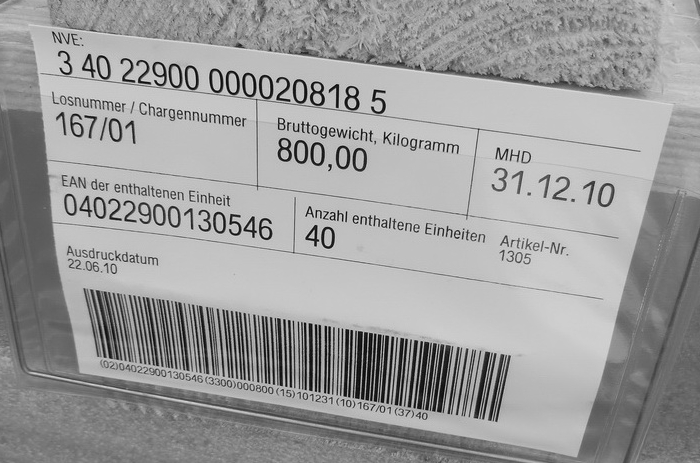
\includegraphics[width=\columnwidth]{img/techniques/candidate-extraction/grayscale}
    \caption{\scriptsize Grauwerte}
  \end{subfigure}
  \begin{subfigure}[t]{.32\columnwidth}
    \centering
    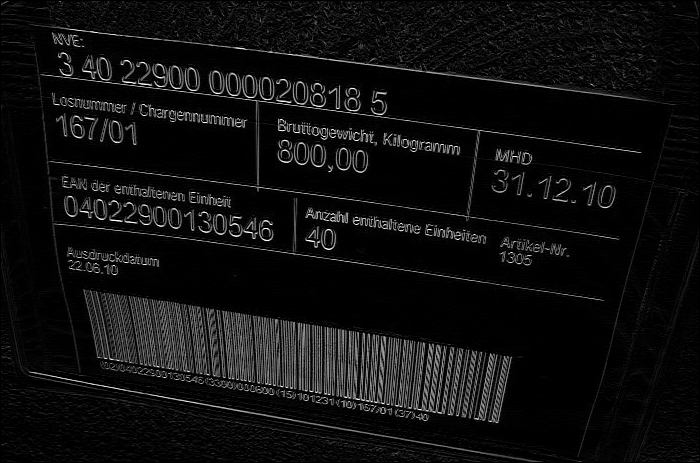
\includegraphics[width=\columnwidth]{img/techniques/candidate-extraction/edges}
    \caption{\scriptsize Kantenbild unter Verwendung des \textsc{Roberts}-Operator}
  \end{subfigure}
  \begin{subfigure}[t]{.32\columnwidth}
    \centering
    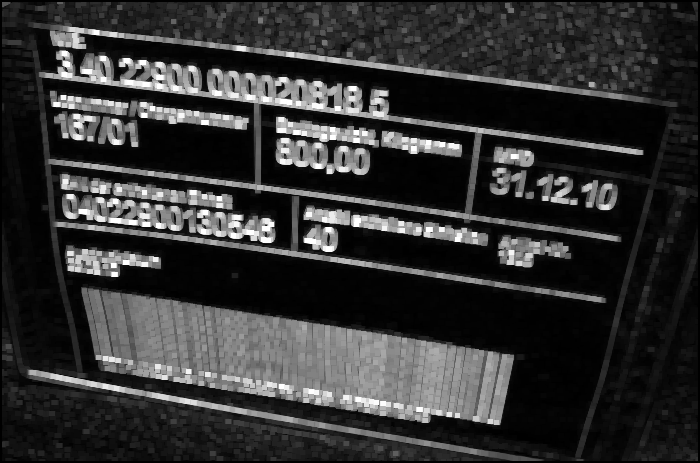
\includegraphics[width=\columnwidth]{img/techniques/candidate-extraction/dilation}
    \caption{\scriptsize Dilation mit einem 5$\times$5-Strukturelement}
  \end{subfigure}
  \begin{subfigure}[t]{.32\columnwidth}
    \centering
    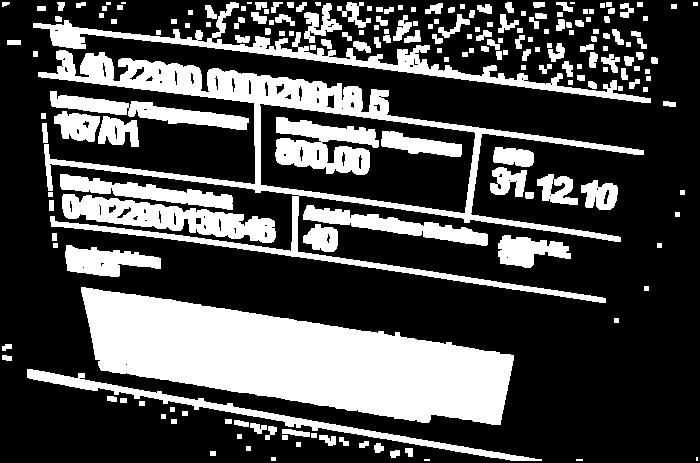
\includegraphics[width=\columnwidth]{img/techniques/candidate-extraction/binary}
    \caption{\scriptsize Binärbild}
  \end{subfigure}
  \begin{subfigure}[t]{.32\columnwidth}
    \centering
    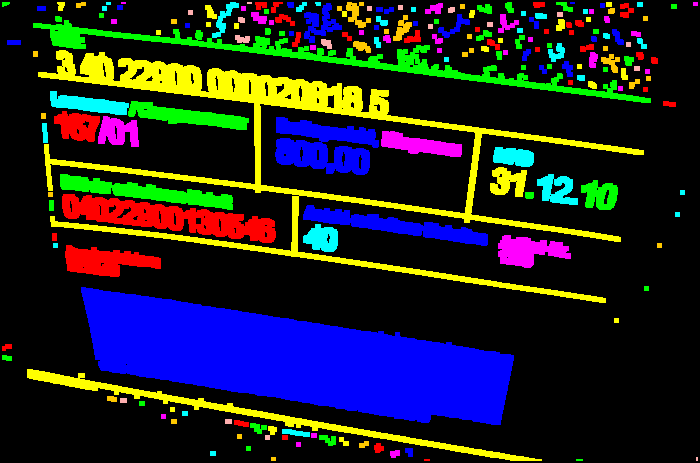
\includegraphics[width=\columnwidth]{img/techniques/candidate-extraction/components}
    \caption{\scriptsize zusammenhängende Komponenten farblich hervorgehoben}
  \end{subfigure}
  \begin{subfigure}[t]{.32\columnwidth}
    \centering
    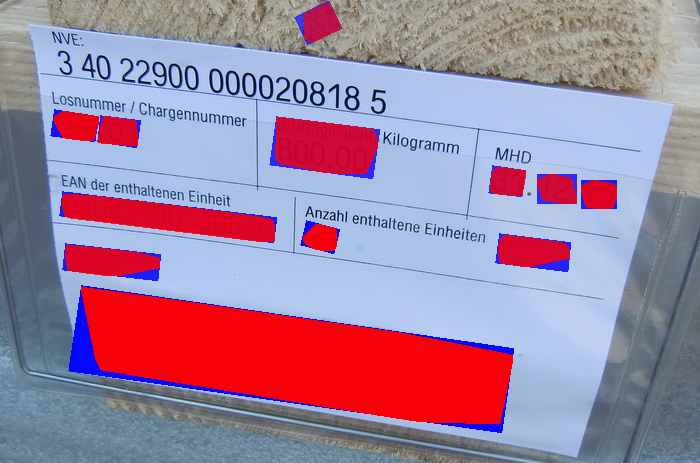
\includegraphics[width=\columnwidth]{img/techniques/candidate-extraction/candidates}
    \caption{\scriptsize ermittelte Regionen (rot) mit umschließendem Rechteck minimaler Fläche (blau)}
  \end{subfigure}
  \caption[Einzelschritte beim Auffinden potentieller Barcodes]{
    Einzelschritte beim Auffinden potentieller Barcodes in einem Bild\protect\footnotemark.
    Bild (f) zeigt deutlich, dass das Verfahren auch Text erfasst.}
\end{figure}

\footnotetext{\url{http://commons.wikimedia.org/wiki/File:Drahtb\%C3\%BCgeltasche_A6.jpg}}

